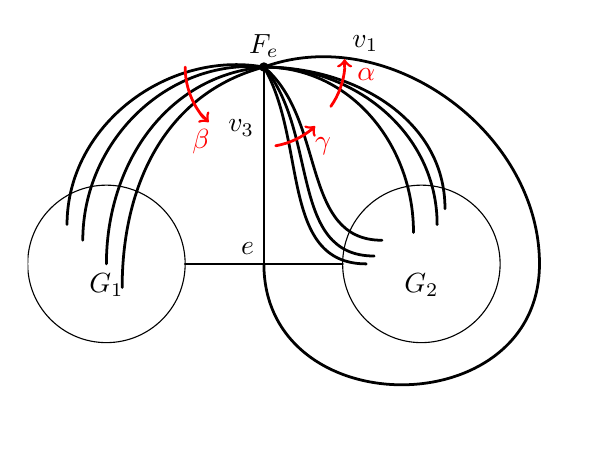
\begin{tikzpicture}[line cap=round,line join=round,x=1cm,y=1cm]
\clip(-1,-2) rectangle (6,3);

\draw (0,0) circle [radius=1cm];
\draw (4,0) circle [radius=1cm];
\draw (0,0) node[anchor=north] {$G_1$};
\draw (4,0) node[anchor=north] {$G_2$};


\draw [line width=1pt] (2,2.5) to[out=170,in=90,looseness=1] (-.5,.5); % F0 -- F2
\draw [line width=1pt] (2,2.5) to[out=175,in=90,looseness=1] (-.3,.3); % F0 -- F2
\draw [line width=1pt] (2,2.5) to[out=185,in=90,looseness=1] (0,0); % F0 -- F2
\draw [line width=1pt] (2,2.5) to[out=195,in=90,looseness=1] (.2,-.3); % F0 -- F2



%e*
\draw [line width=1pt] (2,2.5) to (2,0); % F0 -- F1
\draw [line width=1pt] (2,0) to[out=-90,in=-90,looseness=1.5] (5.5,0); % F0 -- F1
\draw [line width=1pt] (2,2.5) to[out=20,in=90,looseness=1] (5.5,0); % F0 -- F1


\draw [line width=1pt] (2,2.5) to[out=0,in=90,looseness=1] (4.3,.7); % F0 -- F3
\draw [line width=1pt] (2,2.5) to[out=0,in=90,looseness=1] (4.2,.5); % F0 -- F3
\draw [line width=1pt] (2,2.5) to[out=0,in=90,looseness=1] (3.9,.4); % F0 -- F3

\draw [line width=1pt] (2,2.5) to[out=-40,in=180,looseness=1] (3.5,.3); % F0 -- F3
\draw [line width=1pt] (2,2.5) to[out=-50,in=180,looseness=1] (3.4,.1); % F0 -- F3
\draw [line width=1pt] (2,2.5) to[out=-60,in=180,looseness=1] (3.3,.0); % F0 -- F3

% e
\draw [line width=1pt] (1,0) to (3,0); 
\draw (2,0) node[anchor=south east] {$e$};


\draw (2,1.5) node[anchor=south east] {$v_3$};
\draw (3,2.8) node[anchor=west] {$v_1$};


\draw (2,2.5) node[anchor=south] {$F_e$};
\draw [fill=black] (2,2.5) circle (1.5pt);


% Arcos
%\draw (2,2.5) circle [radius=1cm];
\draw[red,line width=1pt] (2.15,1.5) arc (-80:-50:1);
\draw[line width=1pt,->,red] (2.6,1.7) to (2.65,1.75);
\draw (2.75,1.5) node[red] {$\gamma$};


\draw[red,line width=1pt] (2.85,2) arc (-35:-5:1);
\draw[line width=1pt,->,red] (3.025,2.5) to (3.025,2.6);
\draw (3.3,2.4) node[red] {$\alpha$};

\draw[red,line width=1pt] (1,2.5) arc (180:220:1);
\draw[line width=1pt,->,red] (1.2,1.9) to (1.3,1.8);
\draw (1.2,1.55) node[red] {$\beta$};

\end{tikzpicture}
